\documentclass[12pt]{article}

% Use algorithm and algpseudocode packages so \State and related commands are available

\newcommand{\duedate}{---}
\newcommand{\assignment}{Actor-Critic (Lec5) Summary} % Change to "Problem Set X"

% Change the following to your name and UNI.
\newcommand{\name}{Aksel Kretsinger-Walters, adk2164}
\newcommand{\email}{adk2164@columbia.edu}

% NOTE: Defining collaborators is optional; to not list collaborators, comment out the
% line below. Maximum of two collaborators per problem set.
%\newcommand{\collaborators}{Vig Vigerton (\texttt{UNI}), Alice Bob (\texttt{UNI})}
% No collaborators on PS 0

\makeatletter
\def\input@path{{../}{../../}{../../../}} % add as many parents as you need
\makeatother
\input{pset_template_RL.tex} %% DO NOT CHANGE THIS LINE

\begin{document}
\psetheader %% DO NOT CHANGE THIS LINE

\section*{Lecture 4 Summary: Exploration--Exploitation Theory}

\subsection*{Overview}
The exploration--exploitation dilemma is central to reinforcement learning: how to
balance gaining new information (exploration) versus maximizing known rewards (exploitation).
This lecture formalizes that tradeoff through the \emph{multi-armed bandit (MAB)}
framework and explores provably optimal algorithms for regret minimization.

\subsection*{1. The Multi-Armed Bandit (MAB) Problem}
A $K$-armed bandit has $K$ independent actions (“arms”).
At each time $t = 1, 2, \dots, T$:
\begin{itemize}
		\item The learner selects an arm $a_t \in \{1, \dots, K\}$.
		\item Receives a random reward $r_t \sim \nu_{a_t}$ with mean $\mu_{a_t}$.
\end{itemize}

\textbf{Goal:} maximize cumulative reward or equivalently minimize \emph{regret}:
\[
		R_T = T\mu^* - \sum_{t=1}^T \mu_{a_t}, \qquad \mu^* = \max_i \mu_i.
\]
Regret quantifies the cost of exploration—how much reward is lost compared to always
pulling the best arm.

\subsection*{2. Naïve Approaches}

\paragraph{Greedy Algorithm.}
Always choose the arm with highest sample mean $\hat{\mu}_i$.
Fails because it may prematurely exploit a suboptimal arm due to early noise.

\paragraph{$\epsilon$-Greedy.}
With probability $\epsilon_t$, explore randomly; otherwise exploit:
\[
		a_t =
		\begin{cases}
				\text{uniform random arm}, & \text{with prob. } \epsilon_t,\\[4pt]
				\arg\max_i \hat{\mu}_i, & \text{with prob. } 1-\epsilon_t.
		\end{cases}
\]
Typically $\epsilon_t$ decays over time (e.g., $\epsilon_t = 1/t$).
Simple, but not optimal.

\subsection*{3. Optimism in the Face of Uncertainty}

A more principled strategy: select arms using \textbf{Upper Confidence Bounds (UCB)}.

\paragraph{UCB1 Algorithm (Auer et al., 2002).}
At time $t$, choose
\[
		a_t = \arg\max_i \!\left( \hat{\mu}_i + \sqrt{\frac{2 \log t}{n_i}} \right),
\]
where $n_i$ is the number of times arm $i$ has been pulled.

This embodies the idea of \emph{optimism under uncertainty}: each arm’s estimate is
inflated by a confidence bonus that decreases as $n_i$ grows.

\paragraph{Regret Bound.}
\[
		\mathbb{E}[R_T] = O\!\left(\sum_{i:\Delta_i>0} \frac{\log T}{\Delta_i}\right),
		\qquad \Delta_i = \mu^* - \mu_i.
\]
This is provably near-optimal (Lai \& Robbins, 1985).

\begin{figure}[htbp]
		\centering
		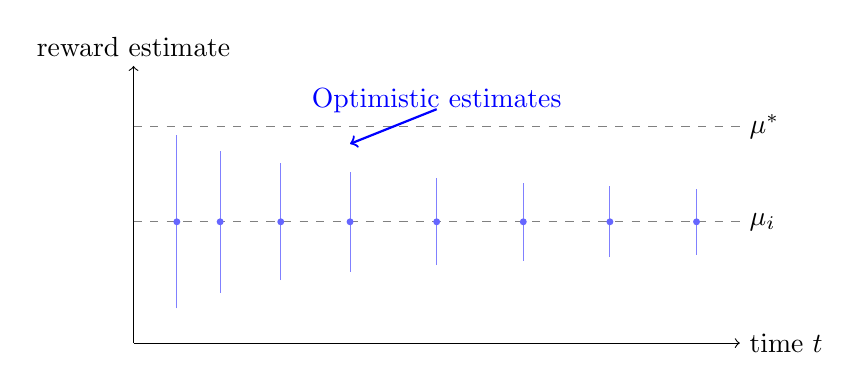
\begin{tikzpicture}[scale=1.1]
				% axes
				\draw[->] (0,0) -- (7,0) node[right] {time $t$};
				\draw[->] (0,0) -- (0,3.2) node[above] {reward estimate};

				% mean lines
				\draw[dashed, gray] (0,2.5) -- (7,2.5) node[right,black] {$\mu^*$};
				\draw[dashed, gray] (0,1.4) -- (7,1.4) node[right,black] {$\mu_i$};

				% confidence intervals
				\foreach \x in {0.5,1,1.7,2.5,3.5,4.5,5.5,6.5}{
						\pgfmathsetmacro{\upper}{1.4 + 1/sqrt(\x+0.5)}
						\pgfmathsetmacro{\lower}{1.4 - 1/sqrt(\x+0.5)}
						\draw[blue!50] (\x,\lower) -- (\x,\upper);
						\fill[blue!60] (\x,1.4) circle (0.04);
				}

				% labels
				\node[blue] at (3.5,2.8) {Optimistic estimates};
				\draw[blue,->,thick] (3.5,2.7) -- (2.5,2.3);
		\end{tikzpicture}
		\caption{Illustration of UCB exploration: each arm’s reward estimate is augmented by a
		shrinking confidence interval.}
\end{figure}

\subsection*{4. Thompson Sampling (Bayesian Bandit)}
A Bayesian alternative maintains a posterior $p(\mu_i|\text{data})$ for each arm:
\begin{enumerate}
		\item Sample $\tilde{\mu}_i \sim p(\mu_i|\text{data})$ for all $i$.
		\item Choose $a_t = \arg\max_i \tilde{\mu}_i$.
		\item Update posterior with observed reward.
\end{enumerate}
This balances exploration and exploitation automatically, achieving the same order of regret as UCB.

\subsection*{5. Lower Bounds on Regret}
\paragraph{Lai \& Robbins Bound (1985).}
Any consistent algorithm satisfies:
\[
		\liminf_{T \to \infty} \frac{\mathbb{E}[R_T]}{\log T}
		\ge \sum_{i:\mu_i < \mu^*} \frac{\Delta_i}{D_{\text{KL}}(\nu_i \,\|\, \nu^*)}.
\]
No algorithm can achieve asymptotically smaller regret.

\subsection*{6. Beyond the Classical Bandit}

\paragraph{Contextual Bandits.}
At each step $t$, an observable context $x_t$ is given, and rewards depend on both $x_t$
and chosen action $a_t$.
Policies $\pi(a|x)$ map contexts to actions.

\paragraph{Linear Bandits.}
Rewards follow $r_t = x_t^\top \theta^* + \eta_t$ with $\|\theta^*\|_2 \le 1$.
The OFUL (Optimism in the Face of Uncertainty for Linear models) algorithm chooses
\[
		a_t = \arg\max_a \left( x_{a,t}^\top \hat{\theta}_t + \alpha_t \|x_{a,t}\|_{V_t^{-1}} \right),
\]
where $V_t = \sum_{\tau<t} x_{a_\tau,\tau} x_{a_\tau,\tau}^\top + \lambda I$.
Regret scales as $O(d\sqrt{T \log T})$ for $d$-dimensional features.

\subsection*{7. Key Takeaways}
\begin{itemize}
		\item Exploration is essential to learn accurate estimates; too little causes bias, too
				much causes inefficiency.
		\item UCB provides a frequentist confidence-based approach with logarithmic regret.
		\item Thompson sampling provides a Bayesian counterpart with similar guarantees.
		\item Contextual and linear bandits generalize exploration--exploitation to structured,
				high-dimensional settings.
\end{itemize}

\end{document}
